\documentclass{article}
\usepackage[utf8]{inputenc}
\usepackage{graphicx}
\usepackage{amsmath}
\usepackage{booktabs}
\usepackage{textcomp}
\usepackage{multirow}
\usepackage{color}

%use (a) for numbering subsections
\renewcommand*\thesubsection{(\alph{subsection})}
\renewcommand*\thesubsubsection{(\roman{subsubsection})}
\title{Aufgabenblatt 3}
\author{Christian Müller, Ralph Krimmel \& Sebastian Albert }

\begin{document}

\maketitle

\section*{Assignment 1 - Fiber Channel, Zoning and FC Topologies}

\subsection{Discuss the advantage of FC-SW over FC-AL}
FC-SW and FC-AL are FC topologies, shown in figure \ref{fig:topo}.

\begin{figure}[h]
	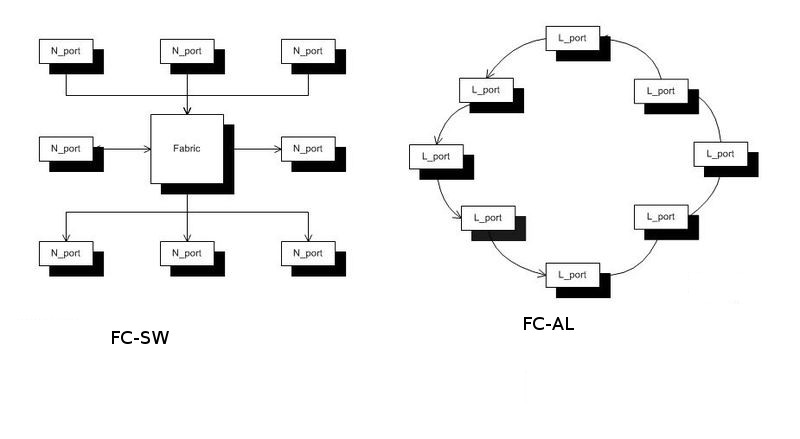
\includegraphics[width=\textwidth]{fctopologies.jpg}
	\caption{FC-SW and FC-AL topologies}
	\label{fig:topo}
\end{figure}

\paragraph{FC-AL}
\begin{itemize}
	\item Means: Arbitrated Loop
	\item Connects up to 127 ports in a ring topology
	\item Just one pair of ports can communicate at a time
	\item One faulty port cuts link, ring not operatable anymore
	\item Hub: Ring topology  but with port bypass circuits
\end{itemize}
	
\paragraph{FC-SW}
\begin{itemize}
	\item Up to $2^24$ Ports can be connected via FC switches (similar to ethernet)
	\item Most performant and reliable implementation of FC
	\item Multiple ports can communicate at one time
	\item Uses always the least loaded path in multi switch environment or multiple ports to one server
	\item No single point of failure (Availability)
\end{itemize}


\newpage
\subsection{How does flow control in a FC network work}
Flow control is the FC-2 control process to pace the flow of Frames between N\_Ports and between an N\_Port and the Fabric to prevent overrun at the receiver. 


Flow control is dependent upon the service classes  

\begin{itemize}
	\item Class 1 Frames use end-to-end flow control: 
		\begin{itemize}
			\item Each frame is acked
			\item Frames are delivered to the destination Port in the same order as they are transmitted
			\item Answer with busy frame when buffer is full
			\item Answer with reject frame if errornous frame received
		\end{itemize}
	\item Class 3 uses only buffer-to-buffer: 
		\begin{itemize}
			\item No acknowledgement of frames 
			\item Destination port sends a Receiver\_Ready primitive signal to the transmitting port whether it has free receive buffers
		\end{itemize}
	\item Class 2 Frames use both types of flow control.
\end{itemize}


\subsection{ What is zoning? Discuss both scenarios}
	Fibre Channel zoning is the partitioning of a Fibre Channel fabric into smaller subsets to: \\
	\begin{enumerate}
		\item Restrict interference
		\item Add security  
		\item Simplify management
	\end{enumerate}

	\subsubsection{ Where is soft zoning prefered over hard zoning?}

	\subsubsection{ Where is hard zoning prefered over soft zoning?}
		
\section{Propose a switched fabric topologie}


\end{document}
